\chapter{Problem definition}
\section{Foreword}
One edge of Medialogy is systems built to react accordingly to humans. This system is called Visual Computing. There are good topics that apply to this kind of technology. One area in which image processing and specific object recognition is used, is surveillance. By implementing some custom made software, one will be able to monitor a specific target group or process. In addition to the semester project two mandatory courses on the third semester of Medialogy are of interest to our semester project.\\
The first course is called Image Processing and it's primarily based on understanding the theory of a picture and tools to manipulate the pixel values within. knowledge such as the principle of 8-bit, the RGB color system, histograms and using threshold to segmentate a picture are some tools learned in the course.\\
The second course used for the semester project is Procedural Programming, in which programming skills in C++ are learned. The theoretical background for programming is necessary to complete image manipulations, based on methods learned in Image Processing.

To structure the semester projects considering supervisors and co-supervisors, every group were asked to discuss which subject field that was of interest to them. In continuation of this, every group were asked to submit an application for the three subjects of the biggest interest, with first, second and third priority.\\
The eleven subjects presented was:

\begin{itemize}
\item Image Processing for Fun Utilizing an Industrial Robot
\item Image Processing for Ambient Intelligent Robots
\item Interactive Floor
\item Interactive Book
\item Interactive Drawing Game
\item Interactive Arcade Game
\item Mobile app for recognizing electric components
\item Emergency system for old people that have fallen
\item Thermal Sock Puppet Show
\item Body Motion Controlled Exercise Game
\item Hjørring Library
\end{itemize}

\section{Establishing collaboration with Hjørring Library}
In continuation of the last subject, Hjørring Library, three groups each year on the third semester are selected to collaborate with Hjørring Library in creating some intuitive interface that will react to humans. It was decided within the group that it was of interest to work with Hjørring Library, therefore an application was sent to the semester coordinator to consider our group as a participant for the library project. This was the first priority of our group. Primarily because it would be a great opportunity for the group to use some of the theory learned in the courses. We considered it a give-and-take experience, as valuable feedback would be given by the staff at the library, but also the visitors. In return the library would be given a project of interest that would encourage their users to visit the library.

As only three groups on the third semester applied for working with Hjørring Library, our group was chosen. A meeting was arranged with Hjørring Library and so together with 5 other groups from third and fifth semester of Medialogy, all groups travelled to Hjørring to meet the library staff. In addition the groups were let loose in the library to check locations for potential projects.\\
After talking to some of the staff, more specific our contact person Martin Jørgensen, some general ideas emerged, so it was decided to go back to the group room at Novi to do some brainstorming within the group.

The first idea that emerged included scanning of barcodes of books in the library. The idea was that the shade of people trespassing the walkway where the canvas was placed would be projected onto the canvas. The conceptual idea was that people would explore the library and depending on the book gathered and loaded, some specific graphic would appear on the canvas. Such as fairy tales from H.C. Andersen that would produce a hat on-top of the user.

After conferencing with the supervisor, Thomas Moeslund, and the co-supervisor, Andreas Møgelmose, it was decided that the conceptual idea needed to be narrowed down to a more specific subject field. The second idea emerged that we should focus mainly on fairy tales and first of all work around H.C. Andersen, which meant adding a hat on-top of the users.

An email was sent to Martin Jørgensen from Hjørring Library concerning the concept for the third semester project, and also about the location for the project. Martin liked the idea, but had some concerns to identify the period in which the project would fit the library. Hjørring Library work around specific topics that change every 8-12 weeks.\fixme{SOURCE NEEDED - maybe from library material} One of the upcoming themes of interest at the library was Christmas that would run from the 2nd week in November until the last week of December. Another idea then emerged in the group towards creating a project for December. Instead of working with the H.C. Andersen theme, it was decided to work with Father Christmas and to add a Christmas hat on top of trespassing users at the library. Martin was fond of this idea and so a new meeting was arranged in order to settle on a suitable location at the library for our project.\\
Two members of the group travelled to Hjørring Library to participate in the meeting with Martin. The outcome was a more specific plan on the project concerning the:

\begin{itemize}
\item The position of the project
\item The equipment that was desired to borrow
\item The light conditions
\end{itemize}

The position of the project will be on the walkway from the reception desk to the core of the library, which Martin believed would be an ideal position for the project, as the light conditions are controllable. In addition to that he knew from experience that people tend to use that walkway either to enter or exit the library, as it is the shortest route. It is placed in the center of the library and is therefore difficult to avoid as a visitor, regardless of whether they are looking for children or adult books.

\begin{figure}[htbp]
\centering
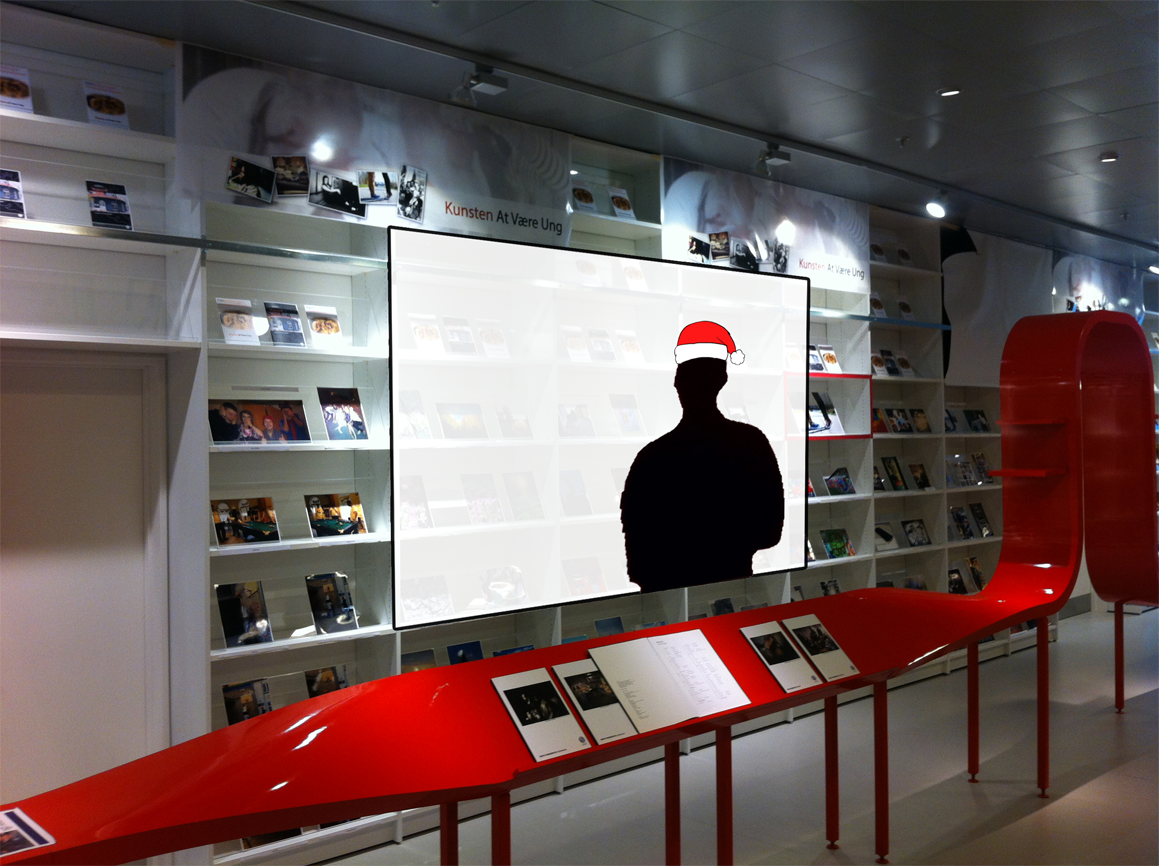
\includegraphics[width=1.00\textwidth]{Pictures/HjoerringLibrary/LocationJohannesHat.jpg}
\caption{Concept art and the location of Hjørring Library}
\label{fig:concept_art}
\end{figure}
Figure \ref{fig:concept_art} illustrates the setup at the library. A canvas with the proportions 3*2.25 meters will be positioned directly on the bookshelves seen in the background of the picture.

\subsection{The initial goal}
One thing that Martin from Hjørring Library was interested in, was knowing the ambitions for the project and what to expect. There had been a talk within the group about ambitions for the project at Hjørring Library. Considering the knowledge in programming and image processing, being ready to present the prototype the 1st of December was a part of the initial goal. Previously Martin told us that the Christmas theme would run from the second week in November, until the last week in December, therefore a 3 week run-time period was a desirable goal.\\
As for the initial goal, Martin expressed his excitement by letting us know that it was very ambitious, but that we should not be intimidated and that he hoped we would succeed. Furthermore he let us know that he would like to contact the designer in charge of the exhibitions at the library to create some interesting scenery for the project. Lastly he expressed that in case we would not succeed to finish the prototype for 1st of December and run for three weeks period, he would like to know, so that he could contact the designer and tell her to do some backup exhibition.

\section{Technical Point of view}
The basic idea is to have a canvas on which the shade of the person is projected together with the Christmas hat added to the top of the head. For that some tools are needed:

\begin{itemize}
\item A web cam to gather input about people trespassing
\item A laptop to run the program code
\item A projector to display the output from the computer
\item A canvas on which the output is projected on
\item Controllable lights/light conditions
\item Power, cables etc.
\end{itemize}

\subsection{Ground zero}
The first step into developing some usable software, was to write some scrappy \fixme{Sounds a little strange - maybe "temporary" or "initial"? - Gustav} code that would run and produce a measurable \fixme{Can we really use it to measure anything? Maybe just "for testing purposes" or "useful output" - Gustav} output. This was done by dividing the entire group consisting of 6 people into 2 smaller groups of 3 people, to come up with a solution on how to produce a segmentation of the video input. Simultaneously a competition

Together with a projector capable of projecting a relative huge output 3*2.25 meters, the laptop running the program code will also be connected to a web cam, modified to collect infrared lightning. This works by having  lamps that projects infrared light, that is "collectable" by the camera. We 

\section{Ultimate goal}
Prototype ready for 1st of December\\
Easy or almost self-maintained
\section{Problem Statement}
      
\textbf{We want an interesting expose at the library that you can enjoy at two different levels. 1) You can walk by and it's funny and 2) you can interact and bring your friends.}\\
\textbf{Easy or almost self-maintained.}

\section{This is awesome}
Yep yep

\begin{figure}[htbp]
\centering
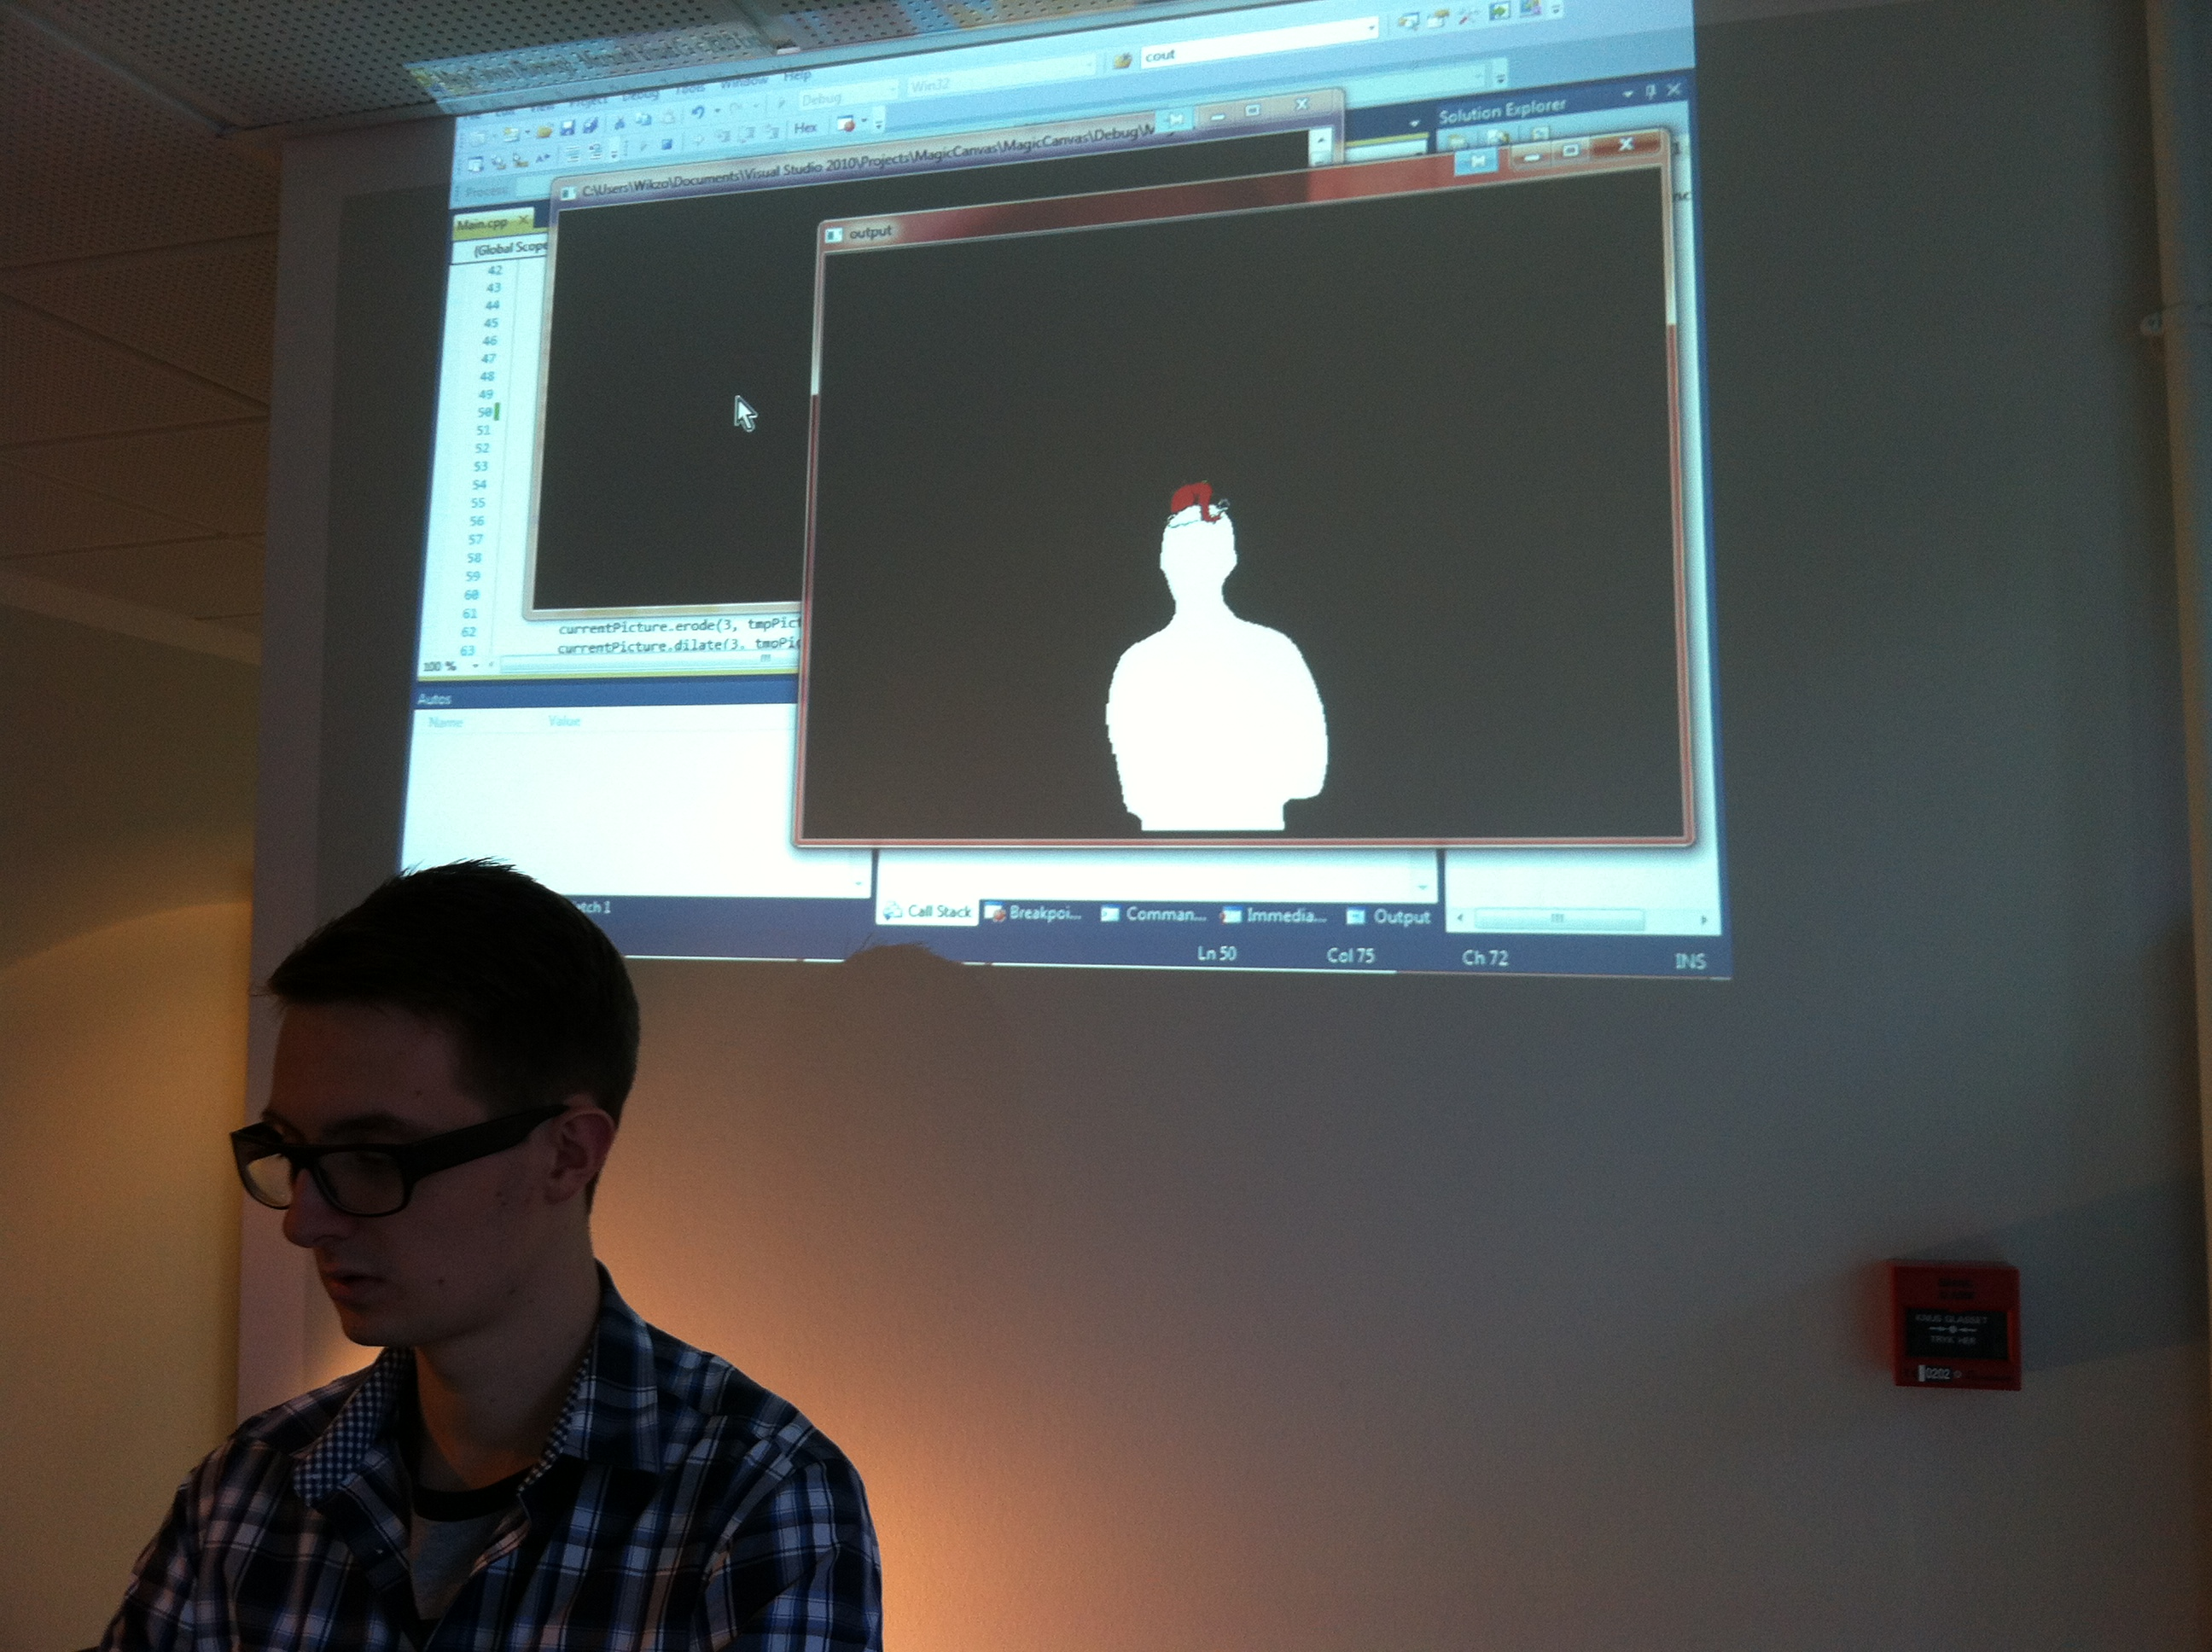
\includegraphics[width=1.00\textwidth]{Pictures/Test/IMG_1477.jpg}
\caption{Picture from Testing the Inferred Camera}
\label{fig:Picture from Testing the Inferred Camera}
\end{figure}

\subsection{Subway is good}
Nah...